\chapter{Test}
Dette kapitel vil indeholde en kort beskrivelse af de tests som er blevet udført i forhold til validering af Rambøll Tilsyn. \\
For den fulde test dokumentation, henvises til Modul- og Integrationstest dokumentet i bilag. \\

\section{Automatiseret test}
I følgende afsnit beskrives unit test der er lavet. Framworket Nunit\cite{NUnit} er blevet brugt til vores testing af klasser. 

\textbf{Validator}
Validator-klassen er en statisk klasse, som har håndterer validering af input felterne i applikationen. Applikationens testcases kan ses på Figur \ref{fig:ValidatorUnit}.
\begin{figure}[H]
	\centering
	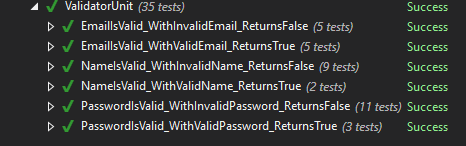
\includegraphics[width=0.6\linewidth]{Test/ValidatorUnit}
	\caption{Screenshot af test sessionen på ValidatorUnit}
	\label{fig:ValidatorUnit}
\end{figure}

En af unit testene, som kan ses på Figur \ref{fig:ValidatorUnit}, er for funktionen PasswordIsValid. Her bliver der testet for både valide og invalide kodeord.\\
Funktionen PasswordIsValid tjekker at et password opfylder disse krav:
\begin{itemize}
	\item Minimum 6 karakter lang
	\item Minimum et stort bogstav
	\item Minimum et lille bogstav
	\item Minimum et tal
	\item Speciel tegn er valgfrit
	\item Må ikke have mellemrum
\end{itemize}

Validator klassen er den eneste klasse der auto testes, fordi at det er den eneste klasse, der indeholder en algorithme. Koden som benyttes i prototypen ligger i forskelllige frameworks og derfor tages der højde for at disse er vel implementeret og gennemtestet. Dette er grunden til at der ikke implementeret mere auto test. 

\clearpage

\section{Manuel test}
I følgende afsnit beskrives de test cases for 'Login' og 'Opret bruger' viewene til Rambøll Tilsyn.

Denne sektion indeholder de manuelle tests for 'Login' og 'Opret bruger' viewene. Der er skrevet tilsvarende test cases for alle de implementerede views. Disse kan findes i Modul- og Integrationstest dokumentets afsnit \ref{Test-sec:ManuelTest}. \\ \\
\textbf{Login tests} \\
\textbf{Pass/fail criteria:} \\
Alle steps skal verificeres på Rambøll Tilsyn applikationen:
\begin{itemize}[-]
	\item Verificer at bruger kan logge ind med korrekte brugeroplysninger.
	\item Verificer at bruger ikke kan logge ind med forkert email.
	\item Verificer at bruger ikke kan logge ind med forkert kodeord. \\
\end{itemize}

\textbf{Opret bruger test} \\
\textbf{Pass/fail criteria:} \\
Alle steps skal verificeres på Rambøll Tilsyn applikationen:
\begin{itemize}[-]
	\item Verificer at en bruger kan oprettes, hvis alle felter er udfyldte korrekt.
	\item Verificer at en bruger ikke kan oprettes, hvis e-mail feltet mangler at blive udfyldt.
	\item Verificer at en bruger ikke kan oprettes, hvis kodeord feltet mangler at blive udfyldt.
	\item Verificer at en bruger ikke kan oprettes, hvis fornavn feltet mangler at blive udfyldt.
	\item Verificer at en bruger ikke kan oprettes, hvis efternavn feltetmangler at blive udfyldt.
	\item Verificer at en bruger ikke kan oprettes, hvis telefonnummer feltet mangler at blive udfyldt.
	\item Verificer at en e-mail skal indeholde et @ for at blive godkendt.
	\item Verificer at kodeordet skal overholde kravene omkring minimum 6 cifre, et stort bogstav, et lille bogstav og et tal.
\end{itemize}

De manuelle tests til Rambøll Tilsyn er med til at sikre at både funktionalitet og flow i applikationen fungerer.